\documentclass[12pt]{article}
\usepackage{amsmath}
\usepackage{amssymb}
\usepackage{graphicx}
\begin{document}
	
\title{PHY 566 Computational Physics Project 2}
\author{Yuanyuan Xu, Matthew Epland, Xiaqing Li, Wesley Cohen}
\maketitle

\section{Introduction}
\indent \indent In our project, we wrote a program to simulate the percolation transition on a lattice with $N \times N$ dimensions. Percolation is the movement of a fluid through a porous material. One example of percolation is water flowing through soil.  

This project has two parts.

\subsection{Part A}
\indent \indent In the first part, we use lattice dimensions of N=5, 10, 15, 20, 30, 50, 80 and averaged the results over 50 simulations. For each lattice dimension, we determined the critical probability $p_c$. We plotted $p_c(N^{-1})$ and extrapolated the results to the infinite size limit $p_c(0)$.

\subsection{Part B}
\indent \indent In the second part, we calculated a fraction where the number of sites in the spanning cluster is divided by the number of occupied sites. The fraction is a function of the probability $p$ above the critical probability $p_c$. The lattice size is fixed at N=100. The results were once again average the results over 50 simulations. The data was then fit to a power-law ansatz curve.

\section{Theory}

\subsection{Part A}
\indent \indent Throughout this problem, we used the random number generator.
 In the first part, each spot in the $N \times N$ lattice is set equal to 0. Then, clusters are created using the random number generator. First, a random number is generated, which determines where in the lattice the first cluster is placed. This lattice point is assigned a value of 1. Next, another random number is chosen, which corresponds to another point in the lattice. If this new lattice point neighbors the point in the lattice that is already occupied, it is assigned a value of 1. Otherwise, a new cluster with value 2 is created.  \newline
 \indent Also, after several spots on the lattice have been filled, if there is more than one cluster neighboring a point, this new sites bridges multiple existing clusters. In this case, the clusters neighboring this point are merged together to form a single cluster. This process is continued until there is a common cluster that touches all four edges of the lattice. \newline
 
\indent Next, $p_c$ is calculated from:

\begin{equation}
	p_c=\frac{\text{number of occupied sites}}{\text{total number of sites}}
\end{equation}

\indent where a larger value of $p_c$ corresponds to a lattice that has fewer unoccupied spots.

\subsection{Part B}
\indent \indent In the second part, for a lattice size of N=100, the following fraction is calculated:

\begin{equation}
F(p>p_c)=\frac{\text{number of sites in spanning cluster}}{\text{number of occupied sites}}
\end{equation}

\indent The power-law ansatz can be written as:

\begin{equation}
F=F_0(p-p_c)^\beta
\end{equation}

where $F$ is the fraction of sites in the spanning cluster, $F_0$ is the initial value of $F$, and $\beta$ is a constant is expected to equal to 5/36. The value of $\beta$ is for two dimensional lattices only.\newline

\indent This equation was used to fit the results for 50 simulations where N=100. This data is plotted in the results section in a log-log plot. From this plot, the slope of the straight line fit was extracted.

\section{Results}

\subsection{Part A}

\begin{figure}[!h]
	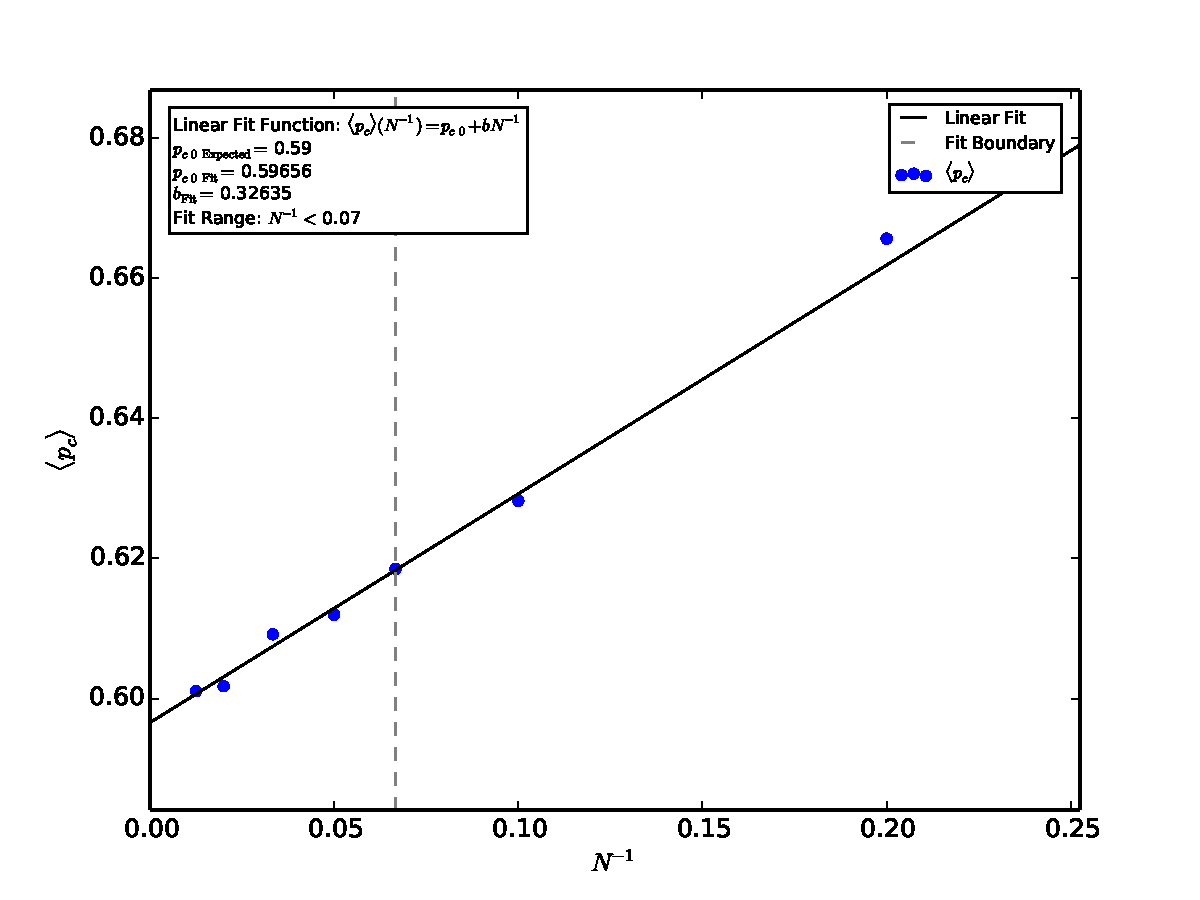
\includegraphics[width=1\textwidth]{../output/plots_for_paper/pc_ave_vs_InverseN.pdf}
		\caption{Critical Probability and Lattice Size Plot}
		\label{fig:1}
\end{figure}

\clearpage
\subsection{Part B}

\begin{figure}[!h]
	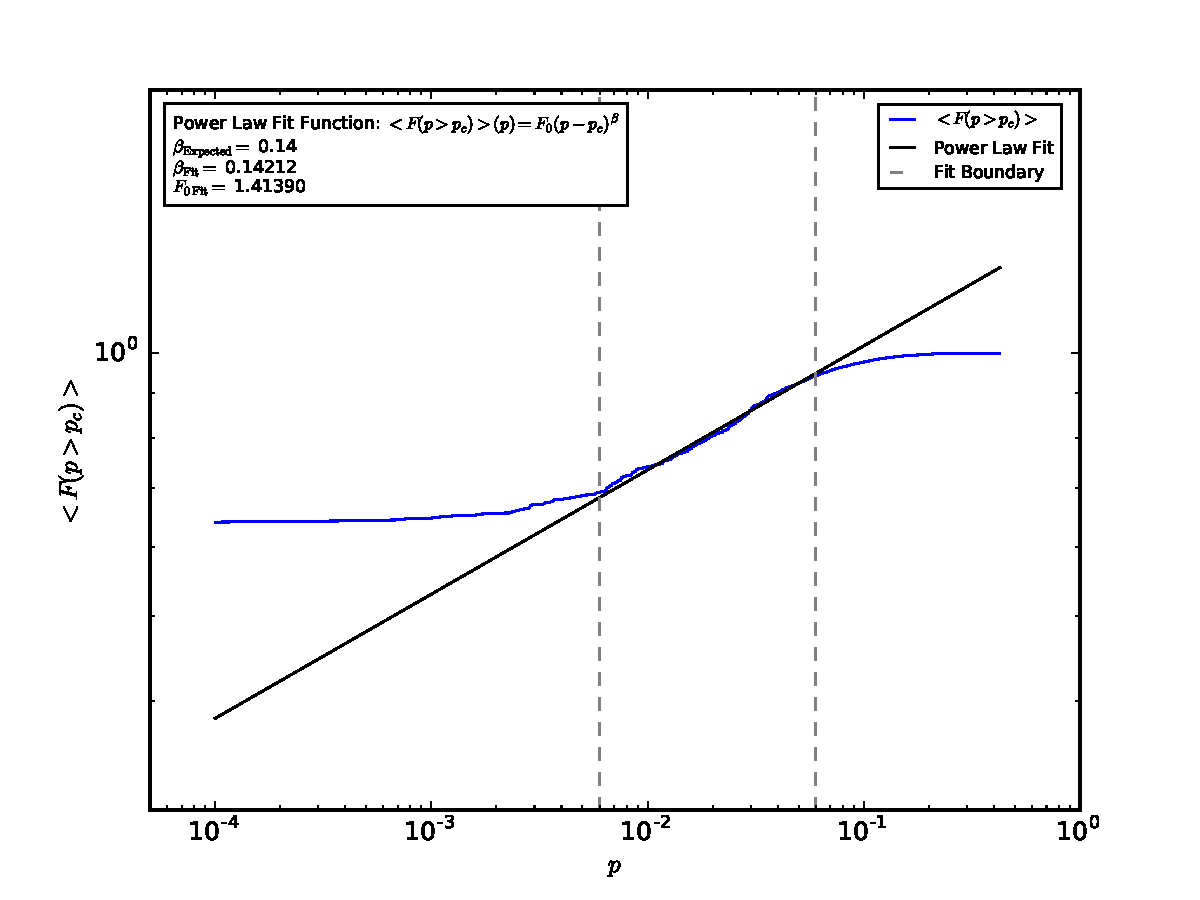
\includegraphics[width=1\textwidth]{../output/plots_for_paper/F_ave_vs_p.pdf}
	\caption{Fraction of Sites and Probability}
	\label{fig:2}
\end{figure}

\section{Discussion}

\subsection{Part A}
\indent \indent The results show that $<p_c>$ increases linearly as $N^{-1}$ increases. The values of $<p_c>$ range from 0.6 to 0.66. The value of $p_c(0)$ the infinite size limit was expected to equal 0.59 and the fit was found to equal 0.59686. The value of $N^{-1}$ ranged from 0 to 0.20.

\subsection{Part B}
\indent \indent The results show that $<F(p>p_c)>$ is on the order of magnitude of $10^0$. The value of $p$ ranges from $10^{-4}$ to $10^0$. The values of the estimated and actual values of $\beta$ are similar. $\beta$ was expected to be 0.14 and the actual value of the fit was 0.14212. From the fit, the value of $F_0$ was determined to be 1.41390.

\end{document}




